\documentclass[letterpaper,11pt]{report}
% Change margins to 1 inch on all sides
\addtolength{\oddsidemargin}{-.875in}
\addtolength{\evensidemargin}{-.875in}
\addtolength{\textwidth}{1.75in}
\addtolength{\topmargin}{-.875in}
\addtolength{\textheight}{1.75in}
\usepackage{float}
\usepackage{graphicx}
\usepackage{footnote}
\usepackage{longtable}
\usepackage{multirow}
\usepackage{tablefootnote}
\usepackage{tabularx}
\usepackage{url}


\DeclareGraphicsExtensions{.pdf,.png,.jpg}

%%%%%%%%%%Start of report
\begin{document} 
\begin{savenotes}
\pagestyle{plain}
\title{CS896 Introduction to Web Science\\Fall 2013\\Report for Assignment 1}
\author{Corren G. McCoy}
 
\date{September 12, 2013}
\maketitle

\renewcommand*\thesection{\arabic{section}}
\setcounter{section}{0}

\setcounter{tocdepth}{4}
\tableofcontents
 \listoffigures
 \listoftables
\newpage


%%%%%%%%%%Chapter Exercises
\section{Assignment 1}
\subsection{Question 1}
\paragraph{Problem}
Demonstrate that you know how to use ``cURL'' well enough to correctly POST data to a form.  Show that the HTML response that is returned is ''correct'' (e.g., save it to a file and then view that file in a browser and take a screen shot).
\paragraph{Response}For this question, the NFL website \url{http://www.NFL.com/} was selected. The page contains a simple form which has a text box that allows the user to search for NFL-related articles using keywords. The following steps were followed to script the HTTP request to POST to the form to initiate the search.
\begin{enumerate}
\item Issued a cURL command to retrieve the HTML source code for the web page which was subsequently saved to a local file on the web server (fast.cs.odu.edu). 
\begin{quote}
curl www.nfl.com -O
\end{quote}
\item Used the Unix grep command to search the local file for all \textless form\textgreater  and \textless input\textgreater tags in order to identify the form field names and the action when the form is submitted.
\begin{quote}
\textless input type=''text'' name=''query'' maxlength=''50'' value=''Search NFL.com'' data-placeholder=''Search NFL.com''/\textgreater
\end{quote}
\item The NFL.com page is a GET form that uses the GET method as shown below.
\begin{quote} 
\textless form class=''ui3-searchbox yui3-skin-sam'' action=''\url{http://search.nfl.com/search}'' method=''get''\textgreater
\end{quote}
\item Issued a query for information concerning ``tim tebow patriots.'' To post to the form, we used the \emph{--data-urlencode} option to send name-value pairs to the website. The urlencode option properly handles our request by replacing spaces with \%20.
\begin{quote}
curl --data-urlencode "query=tim tebow patriots" --location --output nflresults.html "http://search.nfl.com/search"
\end{quote}
\item The \emph{-output} option saves the HTML response to a local file so we can review the result in a browser. Figures \ref{fig:BrowserQuery} and \ref{fig:CURLQuery} show the query results when requested directly from www.NFL.com and the results from the scripted HTTP request. In both instances, we can see the same number of query results (i.e., 34068) in response to the query.
\end{enumerate}

\begin{figure}[htb]
	\centering
		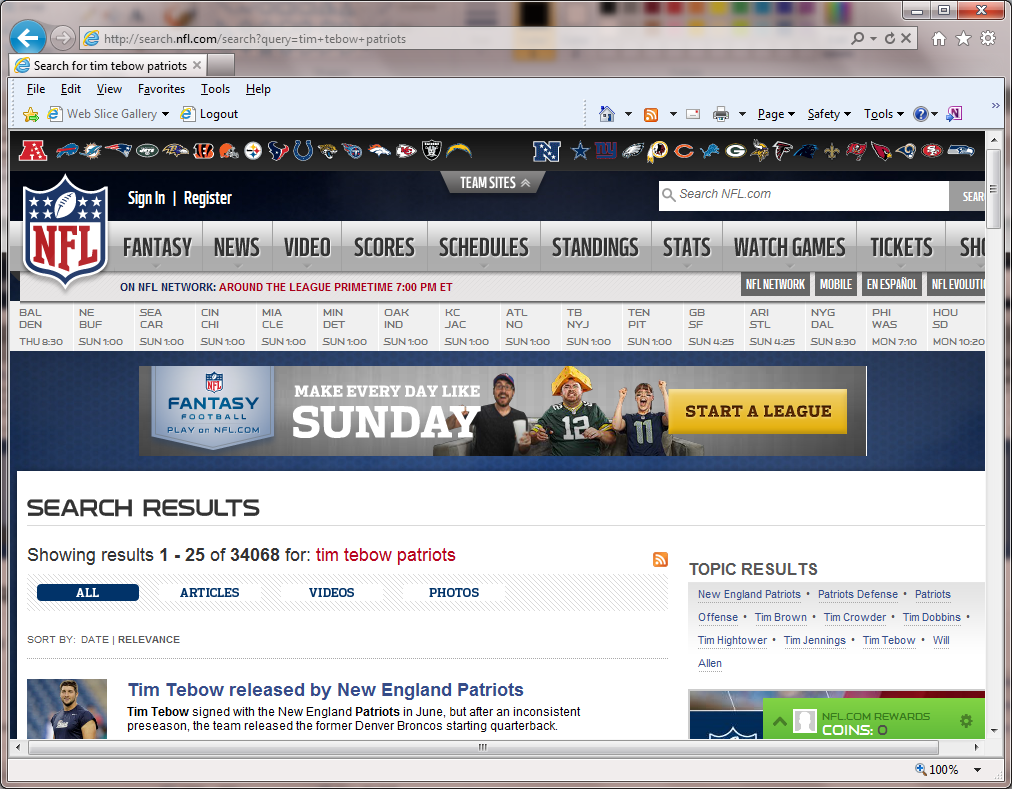
\includegraphics[width=.90\textwidth]{BrowserQuery.png}
	\caption{Browser Query Results}
	\label{fig:BrowserQuery}
\end{figure}

\begin{figure}[htb]
	\centering
		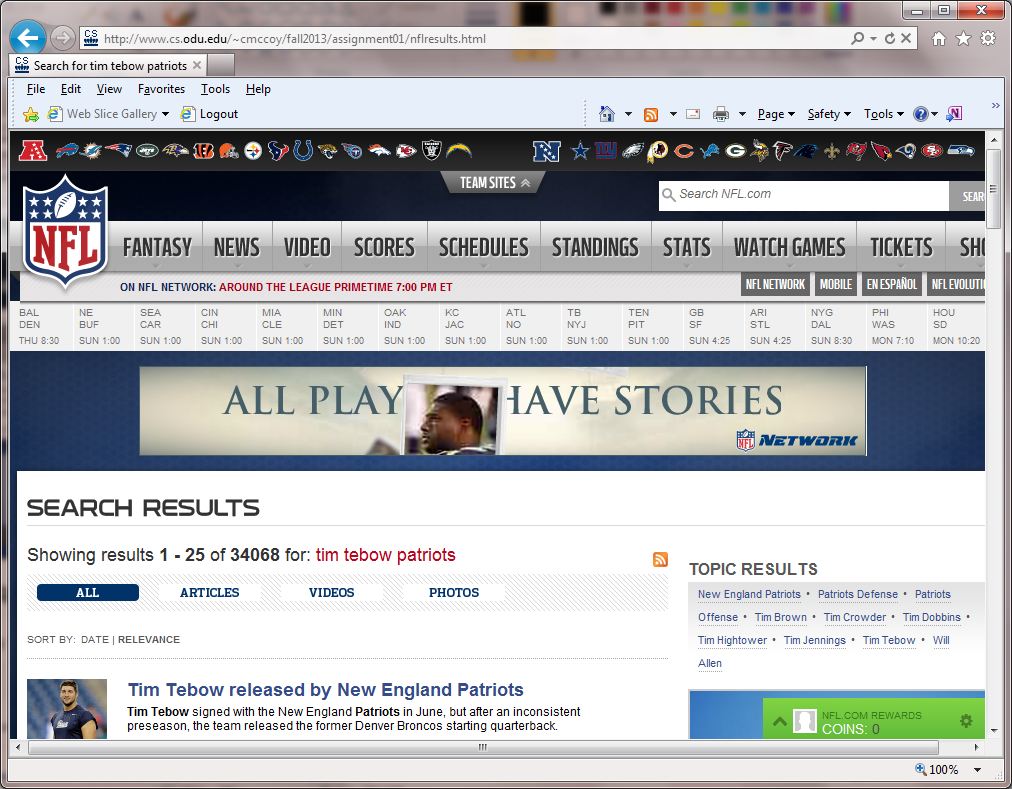
\includegraphics[width=.90\textwidth]{CURLQuery.png}
	\caption{cURL HTML Response}
	\label{fig:CURLQuery}
\end{figure}


%%%%%%%%%%Chapter Exercises
\subsection{Question 2}
\paragraph{Problem} Write a Python program that accepts three arguments: college team, sleep time in seconds, and a URI. The program should download the URI, find the game corresponding to the team argument, print out the current score, sleeps for the specified seconds, and then repeats (until control-C is hit).
\paragraph{Response}We designed a modular program which contains functions that present menus to select a college football team, weekly scoreboard, and prompt the user to enter the sleep time between updates. The user-selected menu options form the arguments for the function that searches the ESPN website (\url{http://scores.espn.go/ncf/scoreboard}) for specific games played during the year and week indicated by the user's selections. In order to efficiently search the website, we first studied the HTML using the \emph{view source} feature in the browser to identify patterns which indicated team pairings and the final score. We discovered the home and visiting team for each game is wrapped in a \textless div\textgreater tag with a class attribute of either \emph{'team visitor'} or \emph{'team home'}. Using the anchor (\textless a\textgreater) tag immediately after the \textless div\textgreater allowed us to extract the name of the football team in each position. We could then iterate over a series of list (\textless li\textgreater) items to locate the final score using a class attribute of \emph{'final'}. Once a pattern was determined, we used the BeautifulSoup (\url{https://pypi.python.org/pypi/BeautifulSoup}) library to parse the HTML and extract the text that we needed (i.e., visiting team, home team). As we navigated through the HTML, we built two parallel lists, indexed by game number, to store each team and final score. Finally, we iterated over the parallel lists, searching for any game where the user's team (e.g., Old Dominion) was either the home or visiting team to display the final score. The source code for our ScoreCenter program is shown in Appendix \ref{chap:Python Source}. A typical user session is shown in Figure \ref{fig:scoreCenterOutput}. No change in score is noted between subsequent updates because no live games were being played.


\begin{figure}[htbp]
	\centering
		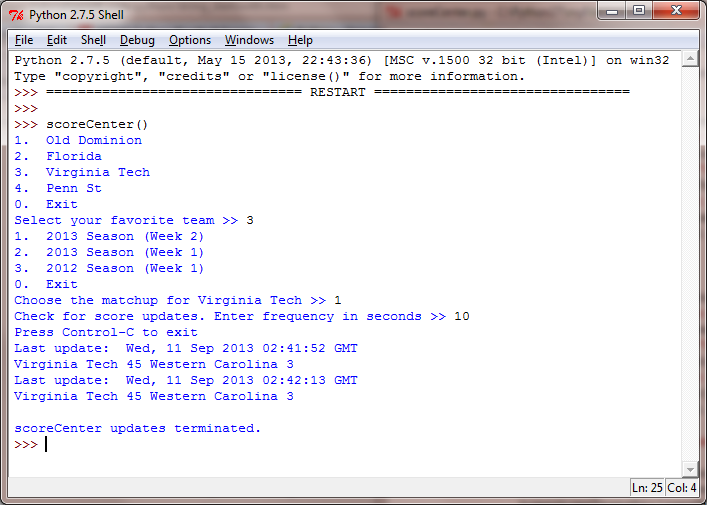
\includegraphics[width=.90\textwidth]{scoreCenterOutput.png}
	\caption{Score Center Session Output}
	\label{fig:scoreCenterOutput}
\end{figure}

%%%%%%%%%%Chapter Exercises
\subsection{Question 3}
\paragraph{Problem}Consider the ``bow-tie'' graph shown in Figure 9 of the Broder et al. \cite{broder2000graph} paper. Now consider the following directed graph whose node connections are described below. Perform a graph analysis as discussed in the referenced paper.
\begin{quote}
A $\rightarrow$ B, B $\rightarrow$ C, C $\rightarrow$ D, C $\rightarrow$ A, C $\rightarrow$ G, E $\rightarrow$ F, G $\rightarrow$ C, G $\rightarrow$ H, I $\rightarrow$ H, I $\rightarrow$ J, I $\rightarrow$ K, J $\rightarrow$ D, L $\rightarrow$ D, M $\rightarrow$ A, M $\rightarrow$ N, N $\rightarrow$ D
\end{quote}

\paragraph{Response}We used the igraph library in R, which is a package for network analysis, to produce graphical representation of the node connections as shown in Figure \ref{fig:Q3-Graph}. The source code which generated the graph is shown in Appendix \ref{chap:R Source}. We then applied the definitions defined in Levene \cite{levene2011introduction} to assign each pair of nodes in the directed graph to a component of the bow-tie structure as shown in Table \ref{tab:bowtie}.

\begin{figure}[htbp]
	\centering
		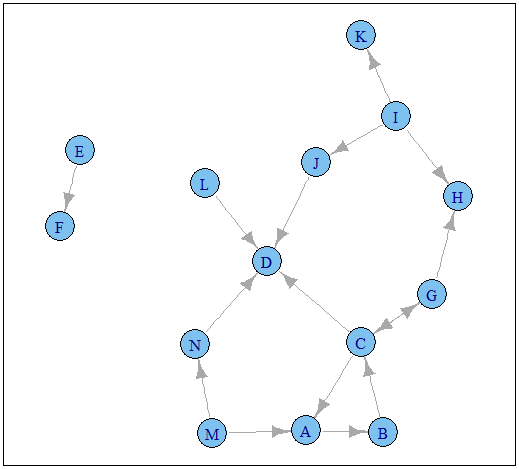
\includegraphics[width=0.90\textwidth]{Q3-Graph.png}
	\caption{Question 3 Graph}
	\label{fig:Q3-Graph}
\end{figure}

\begin{table}
    \begin{tabularx} {1.00\textwidth} {|l|X|X|}
    \hline
    Graph Structure & Characteristic (Levene \cite{levene2011introduction})                                                    & Nodes                         \\ \hline
    IN              & IN consists of pages that can reach the strongly connected component (SCC) but cannot be reached from it. & (M, A)                         \\ \hline
    SCC             & A strongly connected component (SCC) consists of pages that reach one another along directed links.       & (C, A) (A, B) (B, C) (C, G) (G, C) \\ \hline
    OUT             & OUT consists of pages that are accessible from the SCC but do not link back to it.                       & (C, D) (G, H)                  \\ \hline
    Tendrils        & Tendrils contain pages that cannot reach the SCC and cannot be reached from the SCC.                      & (L,D ) (J, D) (I, J) (I, H) (I, K) \\ \hline
    Tubes           & A tube has a directed path from IN to OUT bypassing the SCC.                                             & (M, N) (N, D)                   \\ \hline
    Disconnected    & The pages in the disconnected area are not even weakly connected to the SCC.                             & (E, F)                         \\ \hline
    \end{tabularx}
    \caption {Bow-tie Graph Analysis}
			\label{tab:bowtie}
\end{table}
\end{savenotes}

% produce the bibliography for the citations in your paper.
\bibliographystyle{abbrv}
\bibliography{cmccoy}

\appendix
\addcontentsline{toc}{chapter}{Appendices}

%%Appendix A
\chapter{R Code for Bow-tie Graph} \label{chap:R Source}
\input{graphSource.r}
\chapter{Python Code for ScoreCenter} \label{chap:Python Source}
\input{scoreCenterSource.py}
\end{document} 
%%%%%%%%%%Ed of report
